\tikzset{
block/.style = {draw, fill=white, rectangle, minimum height=3em, minimum width=3em},
tmp/.style  = {coordinate}, 
sum/.style= {draw, fill=white, circle, node distance=1cm},
input/.style = {coordinate},
output/.style= {coordinate},
pinstyle/.style = {pin edge={to-,thin,black}
}
}

\begin{figure}[!htb]
\centering

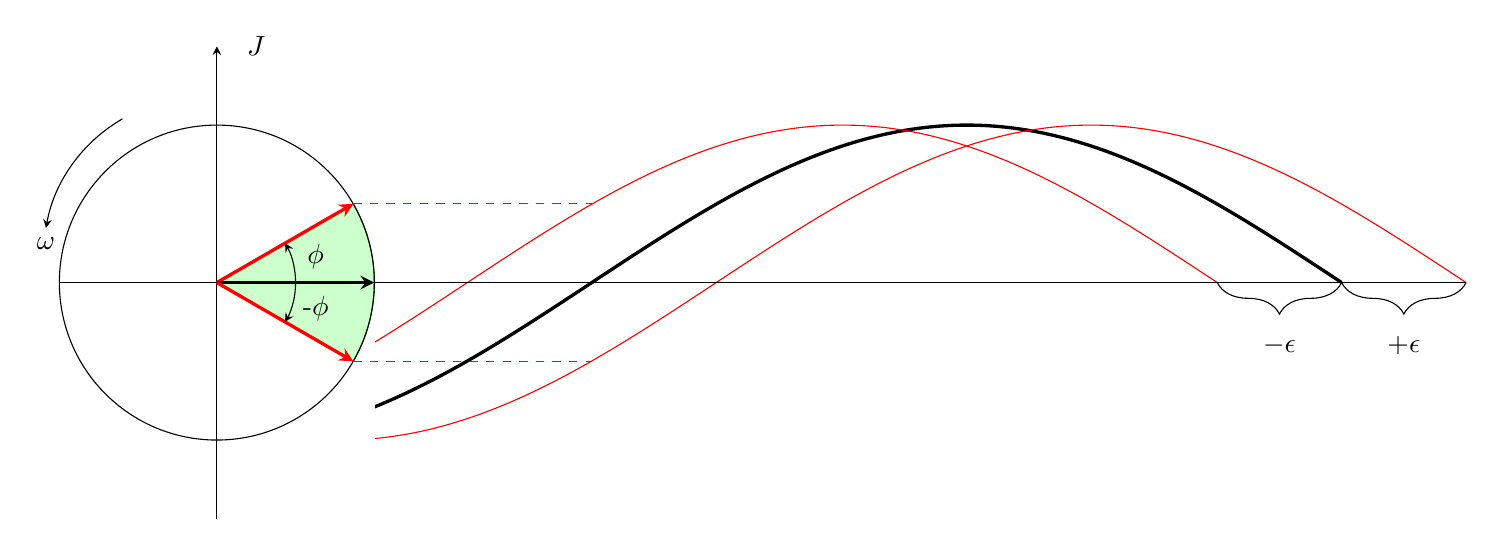
\begin{tikzpicture}
    
    \draw[black,very thick] (0,-2) cos (4.76175,0) sin (2*4.76175,2) cos (3*4.76175,0) ;
    
    \draw[red] (-1.58,-2) cos (4.76175-1.58,0) sin (2*4.76175-1.58,2) cos (3*4.76175-1.58,0) ;
    
    \draw[red] (1.58,-2) cos (4.76175+1.58,0) sin (2*4.76175+1.58,2) cos (3*4.76175+1.58,0) ;
    
    \draw [decorate,decoration={brace,amplitude=0.4cm},xshift=0,yshift=0pt]
(3*4.76175+1.58,0) -- (3*4.76175,0) node [black,midway]{};
    \node at (3*4.76175+0.5*1.58,-0.8) {$+\epsilon$};
    
    \draw [decorate,decoration={brace,amplitude=0.4cm,mirror},xshift=0,yshift=0pt]
(3*4.76175-1.58,0) -- (3*4.76175,0) node [black,midway]{};
    \node at (3*4.76175-0.5*1.58,-0.8) {$-\epsilon$};

    \draw [fill opacity=1, fill=white,white] (-1.58,0.1) rectangle(2,-2.1);
    
    \filldraw[fill=green!20!white, draw=green!50!black]
    (0,0) -- (-30:2) arc (-30:30:2) -- cycle;
    \draw (0,0) circle (2cm);
    
    \draw[->,-stealth,color=black] (0,-3) -- (0,3);
    \node at (0.5,3) {$J$};
    
    \draw(-2,0) -- (3*4.76175+1.58,0);
    
    \draw[->,color=red, very thick,-stealth] (0,0)--(30:2);
    \draw[->,color=black, very thick,-stealth ] (0,0)--(0:2);
    \draw[->,color=red, very thick,-stealth ] (0,0)--(-30:2);
    
    \draw[-,color=red, dashed] (30:2)--(4.76175,1);
    \draw[-,color=red, dashed] (-30:2)--(4.76175,-1);
    
    \draw[->,-stealth ]  (0:1cm) arc (0:30:1cm);
    \draw[->,-stealth ]  (0:1cm) arc (0:-30:1cm);
    
    \node at (15:1.3) {$\phi$};
    \node at (-15:1.3) {-$\phi$};
    % angular velocity \omega
    \draw[->,-stealth ]  (120:2.4cm) arc (120:170:2) node[below] {$\omega$};
    
    \end{tikzpicture}
\caption{A scale drawing of the tolerances required for successful phase lock of the GPS $L_1$ signal.The phase, $\phi$ of the locally generated carrier (red) needs to remain within $30\degree$ of the phase the incoming carrier (black). This equates to a $\Delta$ range of 1.58 cm to the satellite.} \label{fig:PhaseDelay}
\end{figure}
